
\dev{Sorci Émile, Marin Malory}{\cite{HennessyPatterson12}}

\textit{
Ce développement présente la construction d'un additionneur rapide : l'additionneur à retenue anticipée (carry-lookahead adder). Ce développement est parfait pour présenter un circuit combinatoire complexe, illustrant la leçon \ref{L19}. De plus, ce circuit utilise un paradigme diviser-pour-régner, illustrant ainsi la leçon \ref{L12} en présentant une implémentation matérielle d'un algorithme. Enfin, ce circuit illustre la manière dont les opérations arithmétiques sont réalisées en machine, et illustre ainsi certains principes de fonctionnement des ordinateurs, illustrant la leçon \ref{L20}. }



\paragraph{Introduction.} Un additionneur $n$ bits est un circuit combinatoire : il peut être écrit sous le forme d'une formule logique. L'additionneur classique (\textit{full-adder}) présente un problème majeur : pour calculer le $i$-ème bit du résultat, on doit attendre la retenue sortante $c_i$. Dans ce circuit, le chemin critique est alors de taille $\mathcal{O}(n)$.\newline

\textit{
On pourra ici dessiner un full-adder et surligner le chemin critique de longueur $n$.
}

\begin{equation}
s_i = a_i\overline{b_i}\overline{c_i} + \overline{a_i}b_i\overline{c_i} + \overline{a_i}\overline{b_i}c_i + a_ib_ic_i
\end{equation}
\begin{equation}
c_{i+1}=a_ib_i+a_ic_i + b_ic_i
\end{equation}

On peut alors réécrire l'équation précédente :
\begin{equation}
c_{i+1}=g_i + p_ic_i,~ g_i=a_ib_i, ~ p_i=a_i+b_i
\end{equation}
\begin{itemize}
\item si $g_i$ est vraie, alors $c_{i+1}$ est vraie, et donc une retenue est \textbf{générée} ;
\item si $p_i$ est vraie, alors si $c_i$ est vraie, alors on a $c_{i+1}$ qui est vraie, la retenue a été \textbf{propagée}.
\end{itemize}

En itérant, on a alors :
\begin{equation}\label{gen}
c_{i+1}=g_i+p_ig_{i-1} + p_ip_{i-1} + p_ip_{i-1}g_{i-2}+....+p_ip_{i-1}...p_1p_0g_0
\end{equation}

\paragraph{CLA.} L'additionneur qui calcule les retenues en utilisant l'équation \ref{gen} s'appelle \textbf{additionneur à retenue anticipée}, ou CLA pour \textit{carry-Lookahead adder}. Malheureusement, cette formule n'est pas utilisable directement telle quelle (il fait faire un {\tt OR} à $n$ entrée et un {\tt AND} à $n$ entrées, et des fils très longs).

On va donc travailler par bloc :
\begin{itemize}
\item $P_{ij}$ : une retenue est propagée de $i$ à $j$.
\item $G_{ij}$ : une retenue est générée entre $i$ et $j$ ;
\end{itemize}

On peut les définir par récurrence de la manière suivante :
\begin{equation}
P_{i,j+1} = P_{i,j}p_{j+1}
\end{equation}
\begin{equation}
G_{i,j+1} = g_{j+1}+ p_{j+1}G_{i,j}
\end{equation}

On a alors pour tout $i\leq j\leq k-1$ :
\begin{equation}
G_{ik} = G_{j+1,k}+P_{j+1,k}G_{ij}
\end{equation}
\begin{equation}
P_{ik} = P_{ij}P_{j+1,k}
\end{equation}
\begin{equation}
c_{j+1} = G_{ij}+P_{ij}c_i
\end{equation}

On peut alors dessiner un additionneur à retenue anticipée sur $4$ bits.

\noindent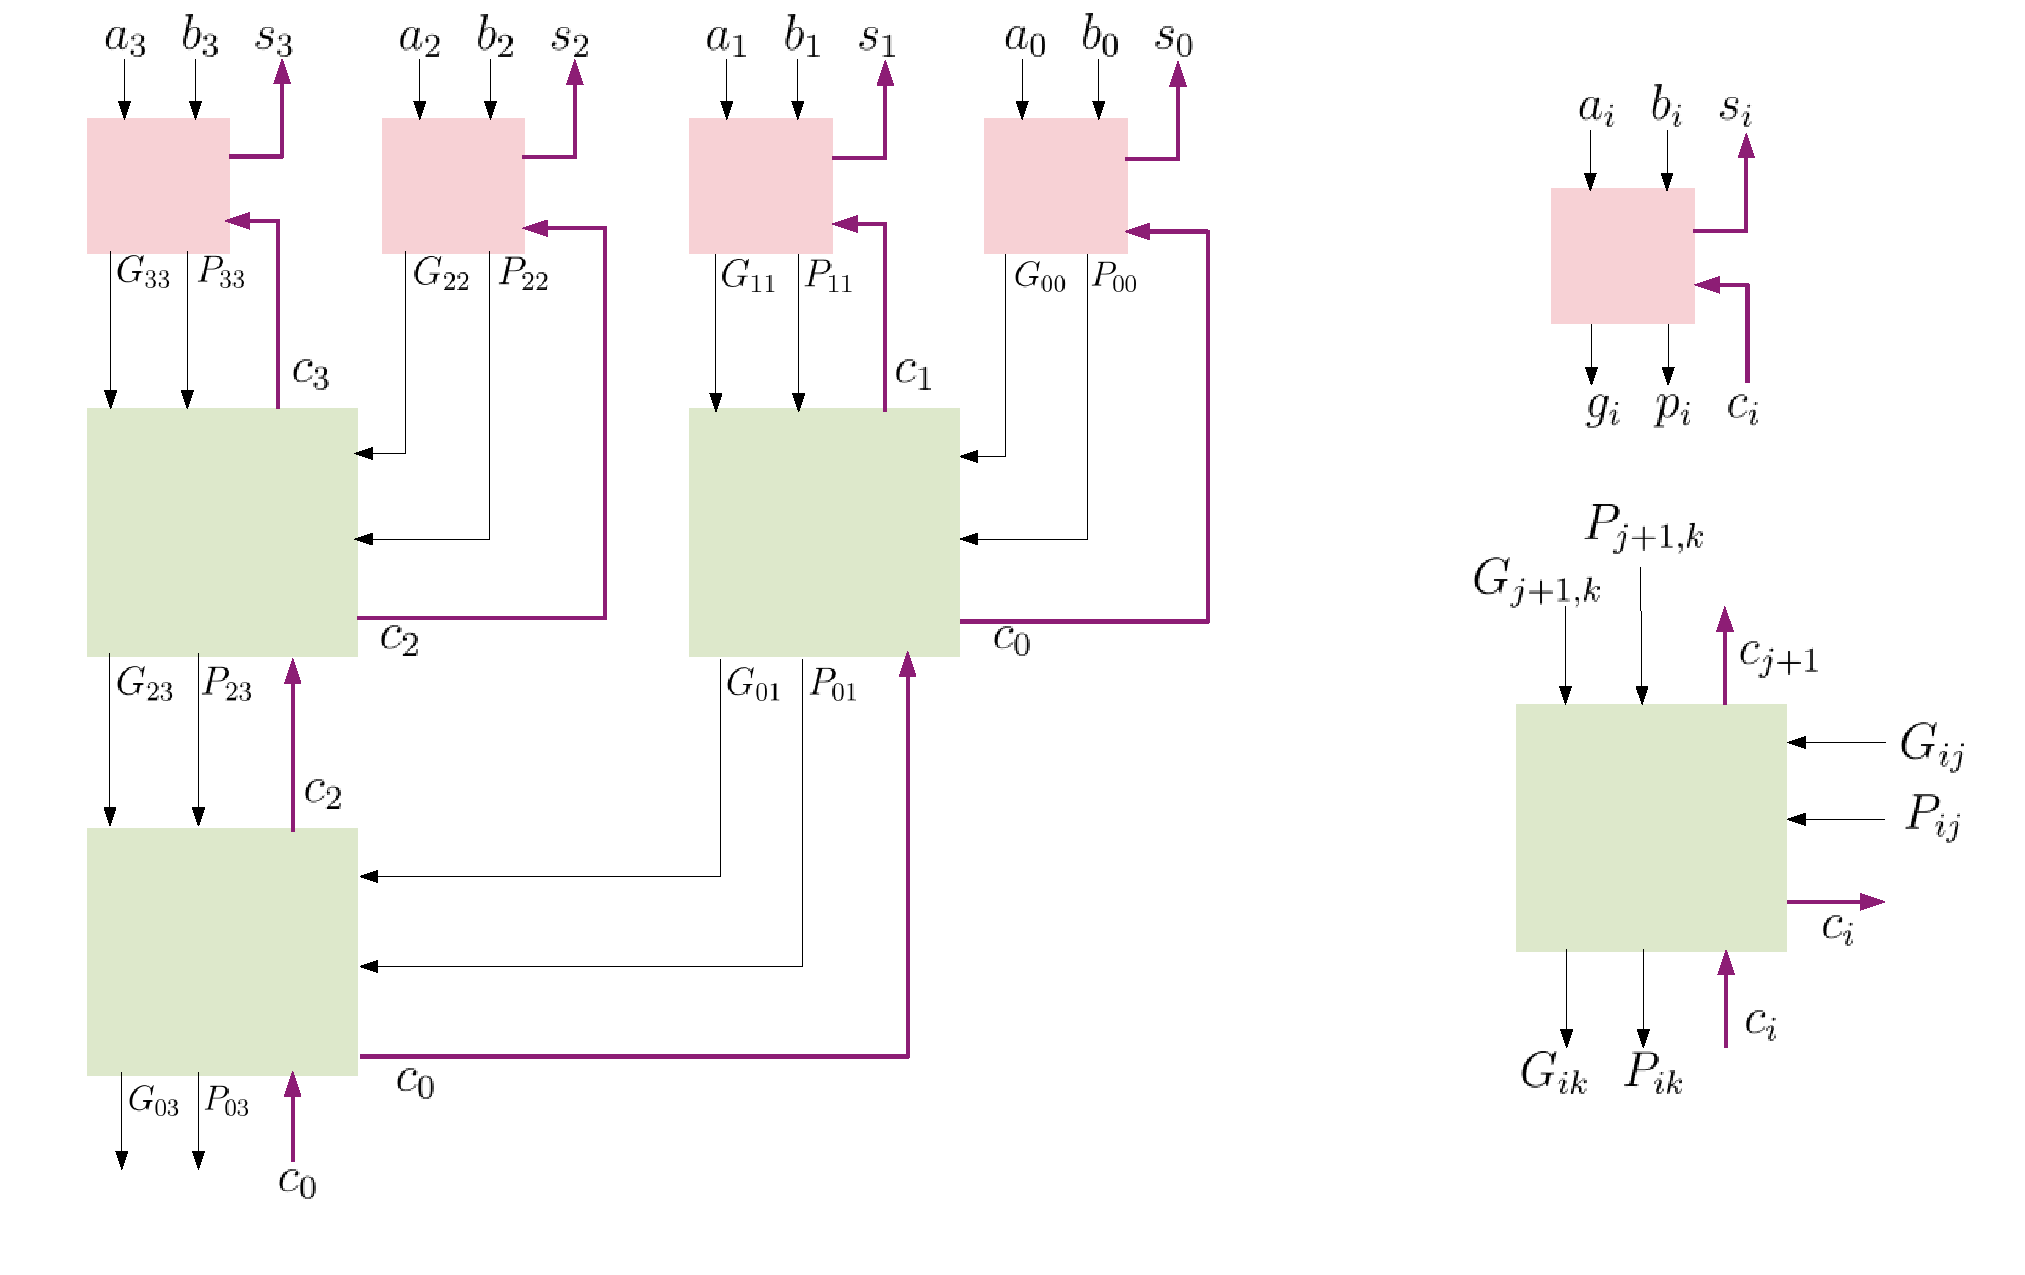
\includegraphics[scale=0.5]{Developpements/Additionneur à retenue anticipée/schéma.pdf} 


En notant $c_v$ et $c_r$ les longueurs des chemins critiques dans dans les blocs vert et rouge, on remarque que pour $n$ bits, la longueur du chemin critique $l_{CLA}(n)$ vérifie l’inéquation :
$$
l_{CLA}(n)= c_v + l_{CLH}(n/2)
$$
et $l_{CLA}(1)=c_r$. Ainsi, on a, on supposant que $n$ est une puissance de $2$ :
$$
l_{CLA} =  \log_2(n)c_v + c_r = \mathcal{O}(\log_2(n))
$$
